%%%%%%%%%%%%%%%%%%%%%%%%%%%%%%%%%%%%%%%%%%%%%%%%%%%%%%%%%%%%%%%%%%%%%%
% Overleaf (WriteLaTeX) Example: Molecular Chemistry Presentation
%
% Source: http://www.overleaf.com
%
% In these slides we show how Overleaf can be used with standard
% chemistry packages to easily create professional presentations.
%
% Feel free to distribute this example, but please keep the referral
% to overleaf.com
%
%%%%%%%%%%%%%%%%%%%%%%%%%%%%%%%%%%%%%%%%%%%%%%%%%%%%%%%%%%%%%%%%%%%%%%

\documentclass[xcolor={dvipsnames}]{beamer}

\mode<presentation>
{
  \usetheme{Madrid}       % or try default, Darmstadt, Warsaw, ...
  \usecolortheme{default} % or try albatross, beaver, crane, ...
  \usefonttheme{default}    % or try default, structurebold, ...
  \setbeamertemplate{navigation symbols}{}
  \setbeamertemplate{caption}[numbered]
}

\usepackage[english]{babel}
\usepackage[utf8x]{inputenc}
\usepackage{graphicx}
\usepackage{hyperref}
  \hypersetup{colorlinks=true}
  \hypersetup{urlcolor=blue}
  \hypersetup{linkcolor = .}
\usepackage{xcolor}
\usepackage{siunitx}
  \sisetup{separate-uncertainty = true}
\DeclareSIUnit\barn{b}
\usepackage{physics}
\usepackage[font=small,labelfont=bf]{caption}
\usepackage{subcaption}
\usepackage[en-GB]{datetime2}
\usepackage{overpic}
\usepackage{feynmp}
\DeclareGraphicsRule{*}{mps}{*}{}
\usepackage{scalerel}
\newcommand{\mylbrace}[2]{\vspace{#2pt}\hspace{6pt}\scaleleftright[\dimexpr5pt+#1\dimexpr0.06pt]{\lbrace}{\rule[\dimexpr2pt-#1\dimexpr0.5pt]{-4pt}{#1pt}}{.}}
\newcommand{\myrbrace}[2]{\vspace{#2pt}\scaleleftright[\dimexpr5pt+#1\dimexpr0.06pt]{.}{\rule[\dimexpr2pt-#1\dimexpr0.5pt]{-4pt}{#1pt}}{\rbrace}\hspace{6pt}}

% Trim in percent
\usepackage{adjustbox}

% No "Figure" prefix
\setbeamertemplate{caption}{\raggedright\insertcaption\par}

% Nice decay amplitude diagrams
\usepackage{amsmath,amssymb,tikz-cd}

% Strike out text
\usepackage[normalem]{ulem}

% For figures with text overlay
\usepackage{overpic}

% Arrows
\usepackage{tikz}
\newcommand{\tikzmark}[1]{\tikz[remember picture] \node[coordinate] (#1) {#1};}

% Colourbox with line breaks
\newcommand{\cbox}[2][lime!20]{%
  \colorbox{#1}{\parbox{\dimexpr\linewidth-2\fboxsep}{\strut #2\strut}}%
}

% Vector arrows
\usepackage[pdftex]{pict2e}

% Checkmark symbol
\def\checkmark{\tikz\fill[scale=0.4](0,.35) -- (.25,0) -- (1,.7) -- (.25,.15) -- cycle;}

% Here's where the presentation starts, with the info for the title slide
\title[Heidelberg tracking meeting]{Resprucing update on tracking efficiencies and A/S week presentation}

\author[Martin Tat]{Martin Tat}
\institute[Heidelberg]{Heidelberg University}
\date{28th April 2026}

\titlegraphic{
\includegraphics[height = 2.3cm]{lhcb.jpg}\hspace{1.0cm}~%
              
\includegraphics[height = 2.3cm]{HeidelbergLogo.pdf}}

\begin{document}

\begin{frame}
  \titlepage
\end{frame}

% These three lines create an automatically generated table of contents.
%\begin{frame}{Outline}
%  \tableofcontents
%\end{frame}

\begin{frame}{Resprucing of 2024 blocks 7 and 8}
  \vspace{0.0cm}
  {\Large A resprucing campaign for 2024 blocks 7 and 8 was performed}
  \vspace{0.2cm}
  \begin{itemize}
    \setlength\itemsep{0.8em}
    \item{No sprucing prescale of $0.4$}
    \item{I have run an AP and added the new samples to TrackCalib2}
    \item{Overall no big surprises}
    \item{Extra stats is nice, especially for MuonUT, but no significant changes}
  \end{itemize}
\end{frame}

\begin{frame}{Before and after resprucing tracking efficiencies}
  \vspace{0.0cm}
  {\large Comparison of tracking efficiencies in all data blocks}
  \begin{figure}[htb]
    \centering
    \begin{subfigure}{0.5\textwidth}
      \centering
      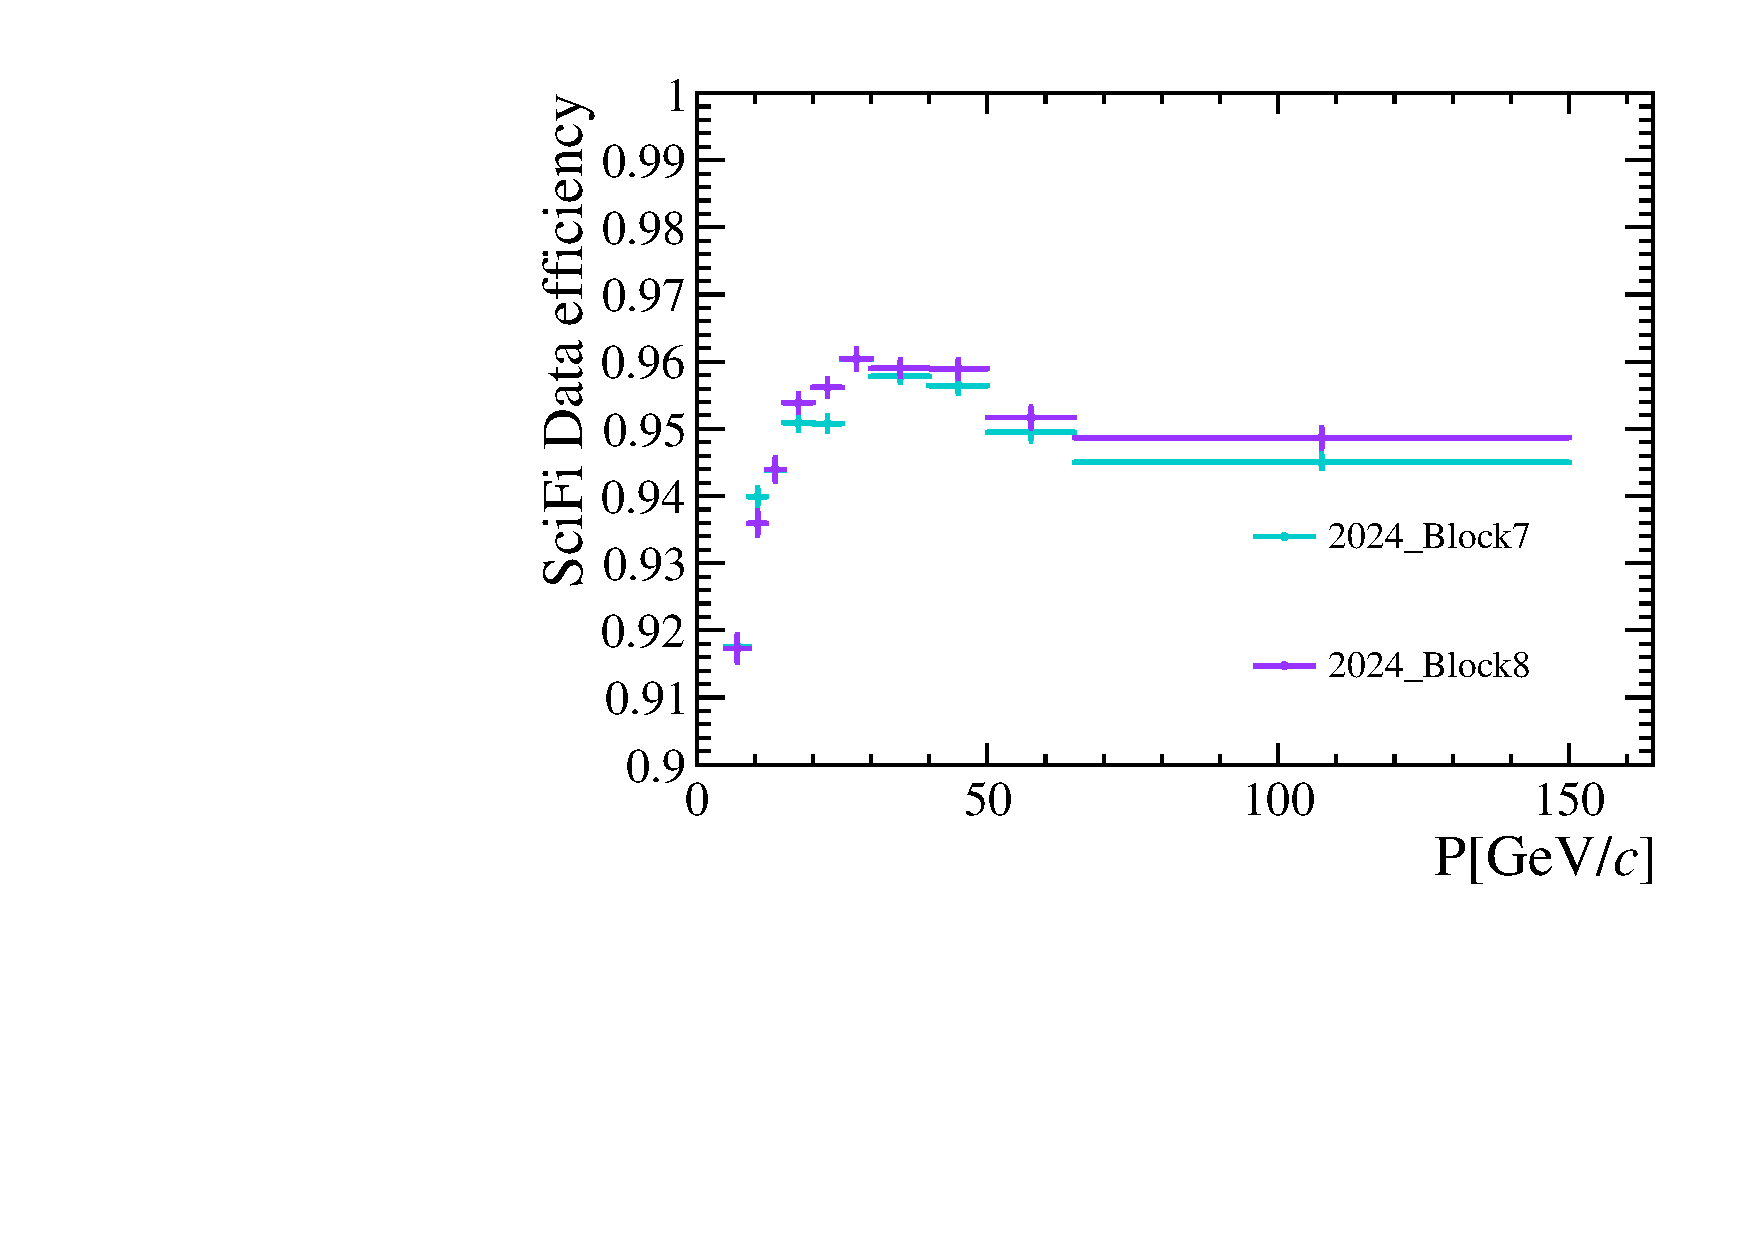
\includegraphics[width=0.75\textwidth]{Plots/trackeff_Data_VeloMuon_P_not_respruced_samples.pdf}
    \end{subfigure}%
    \begin{subfigure}{0.5\textwidth}
      \centering
      
\includegraphics[width=0.75\textwidth]{Plots/trackeff_Data_VeloMuon_P_respruced_samples.pdf}
    \end{subfigure}
    \begin{subfigure}{0.5\textwidth}
      \centering
      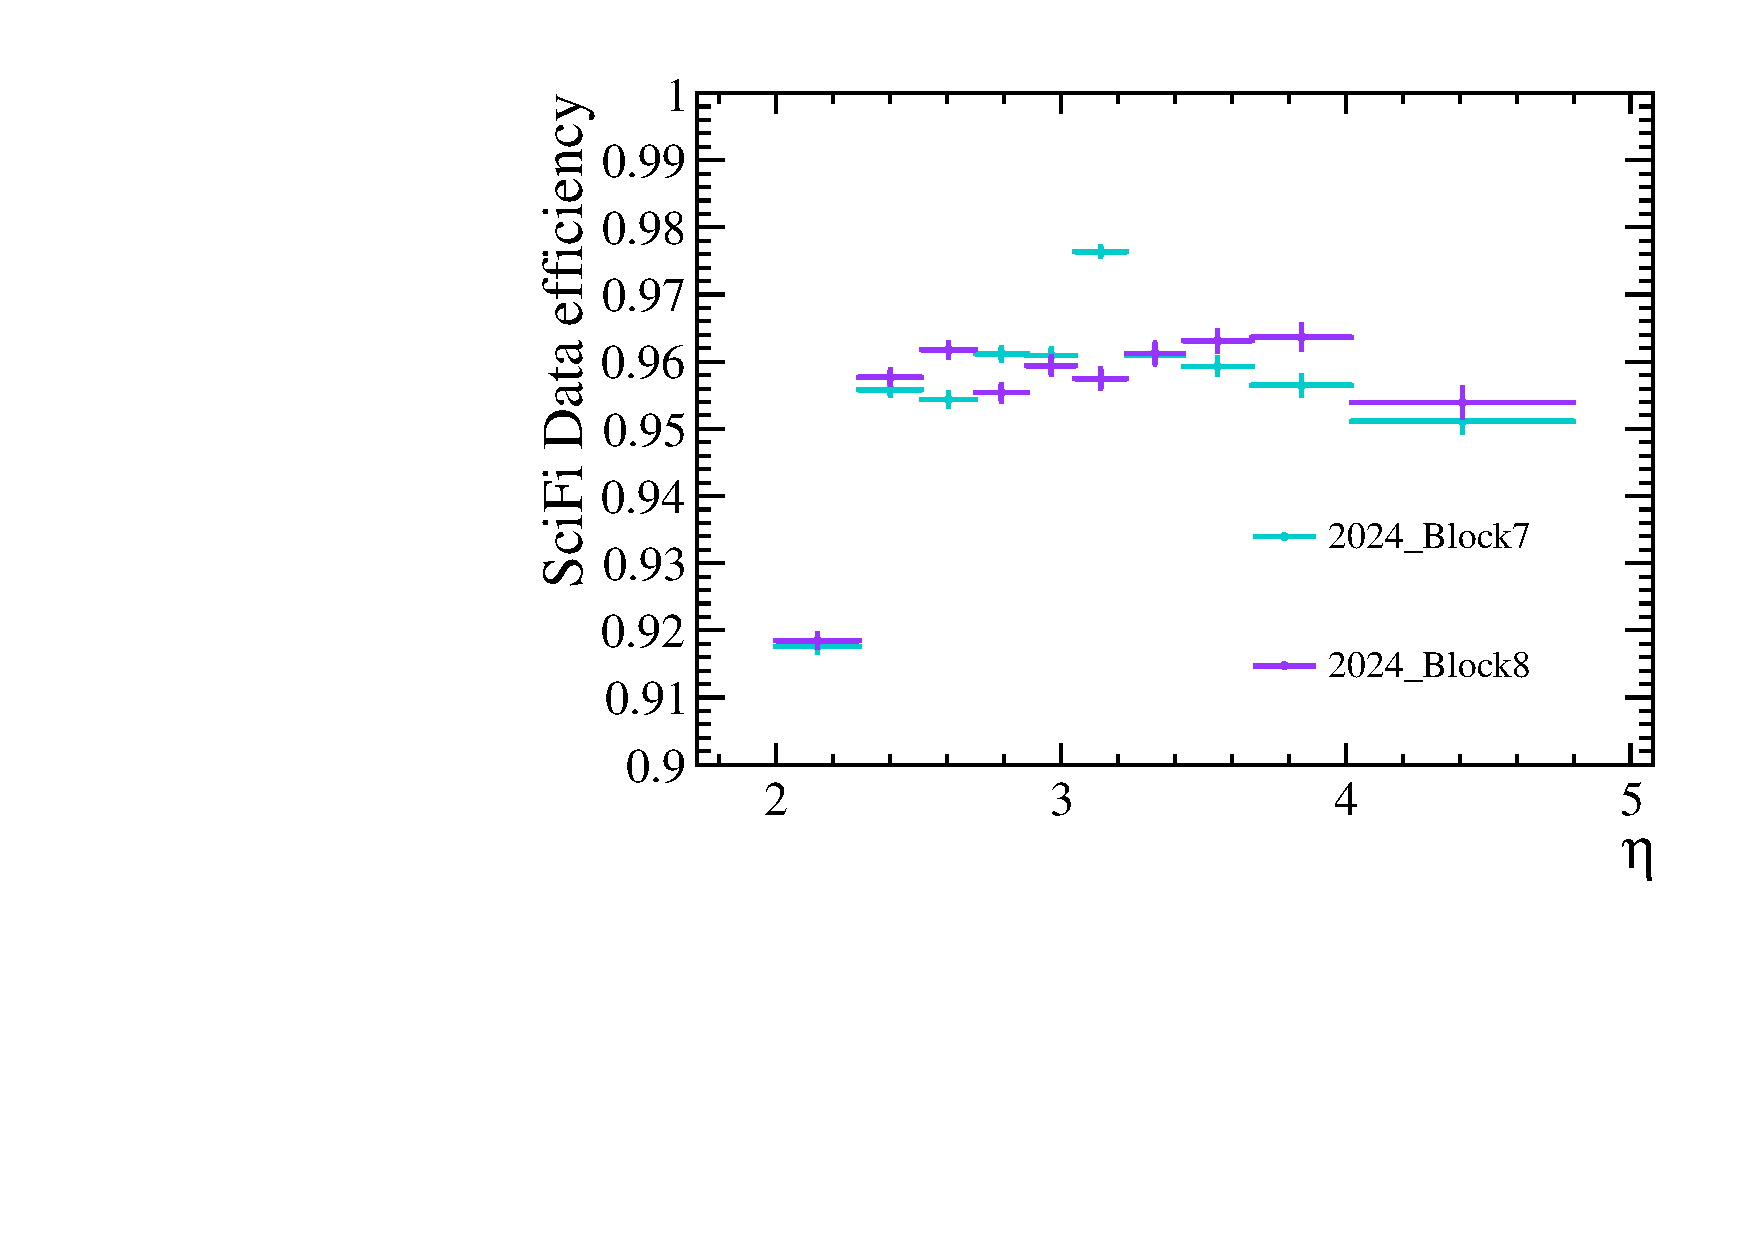
\includegraphics[width=0.75\textwidth]{Plots/trackeff_Data_VeloMuon_ETA_not_respruced_samples.pdf}
    \end{subfigure}%
    \begin{subfigure}{0.5\textwidth}
      \centering
      
\includegraphics[width=0.75\textwidth]{Plots/trackeff_Data_VeloMuon_ETA_respruced_samples.pdf}
    \end{subfigure}
  \end{figure}
  {VeloMuon track efficiencies}
\end{frame}

\begin{frame}{Before and after resprucing tracking efficiencies}
  \vspace{0.0cm}
  {\large Comparison of tracking efficiencies in all data blocks}
  \begin{figure}[htb]
    \centering
    \begin{subfigure}{0.5\textwidth}
      \centering
      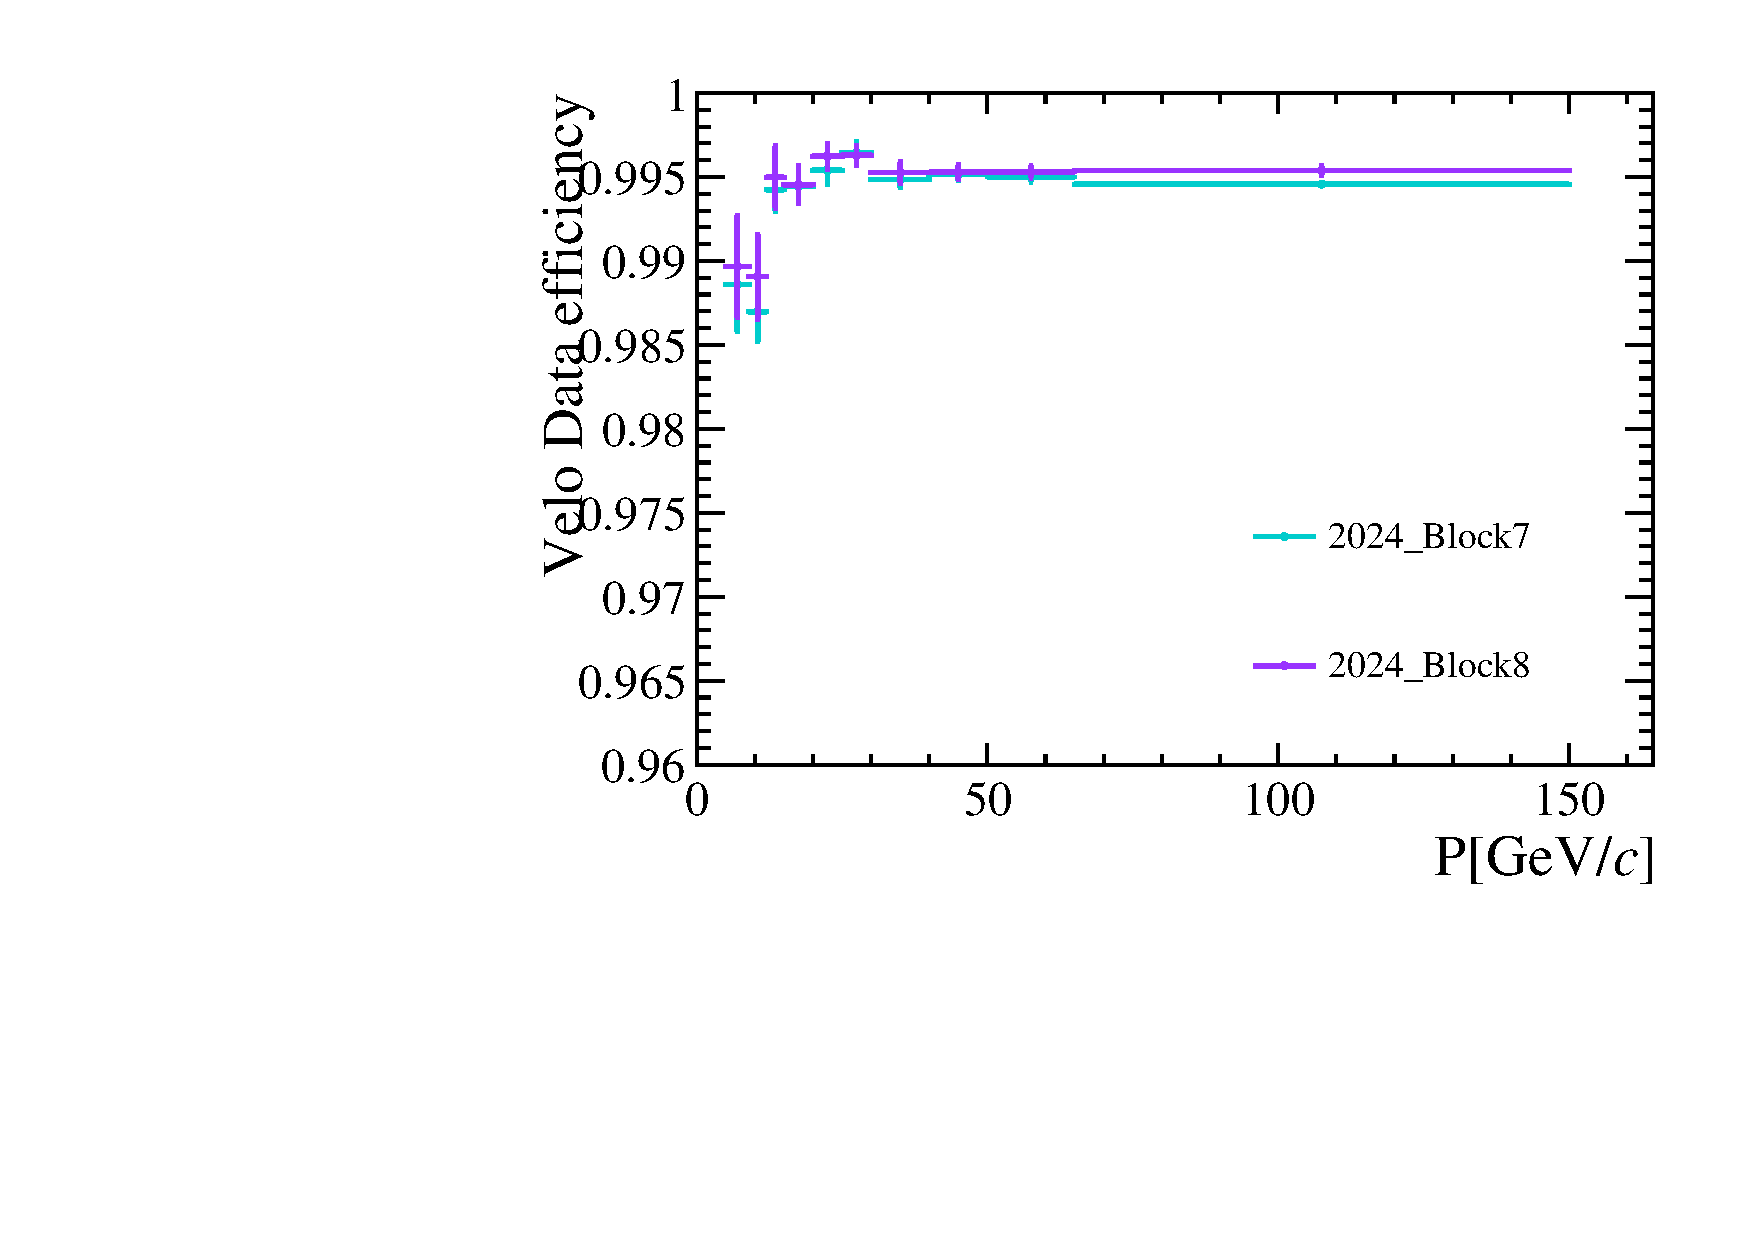
\includegraphics[width=0.75\textwidth]{Plots/trackeff_Data_Downstream_P_not_respruced_samples.pdf}
    \end{subfigure}%
    \begin{subfigure}{0.5\textwidth}
      \centering
      
\includegraphics[width=0.75\textwidth]{Plots/trackeff_Data_Downstream_P_respruced_samples.pdf}
    \end{subfigure}
    \begin{subfigure}{0.5\textwidth}
      \centering
      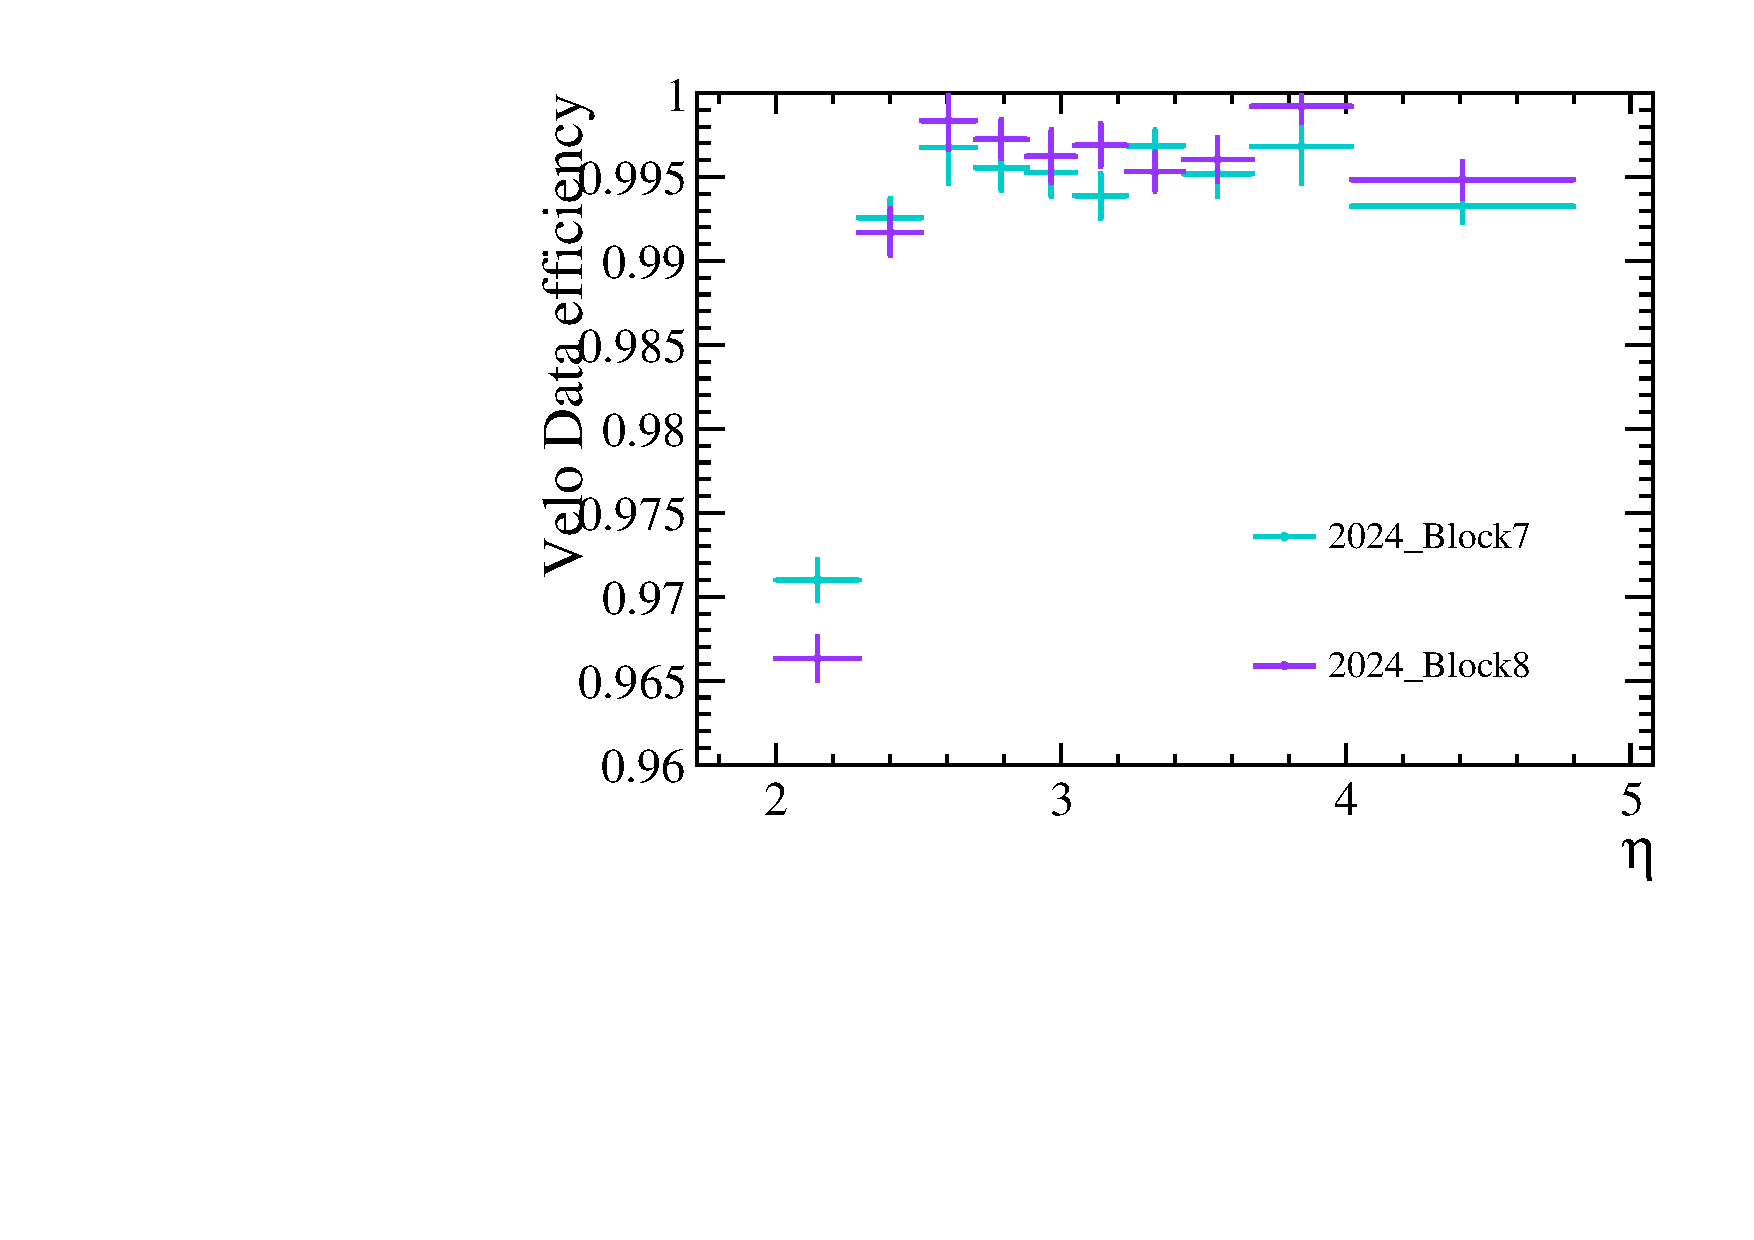
\includegraphics[width=0.75\textwidth]{Plots/trackeff_Data_Downstream_ETA_not_respruced_samples.pdf}
    \end{subfigure}%
    \begin{subfigure}{0.5\textwidth}
      \centering
      
\includegraphics[width=0.75\textwidth]{Plots/trackeff_Data_Downstream_ETA_respruced_samples.pdf}
    \end{subfigure}
  \end{figure}
  {Downstream track efficiencies}
\end{frame}

\begin{frame}{Before and after resprucing tracking efficiencies}
  \vspace{0.0cm}
  {\large Comparison of tracking efficiencies in all data blocks}
  \begin{figure}[htb]
    \centering
    \begin{subfigure}{0.5\textwidth}
      \centering
      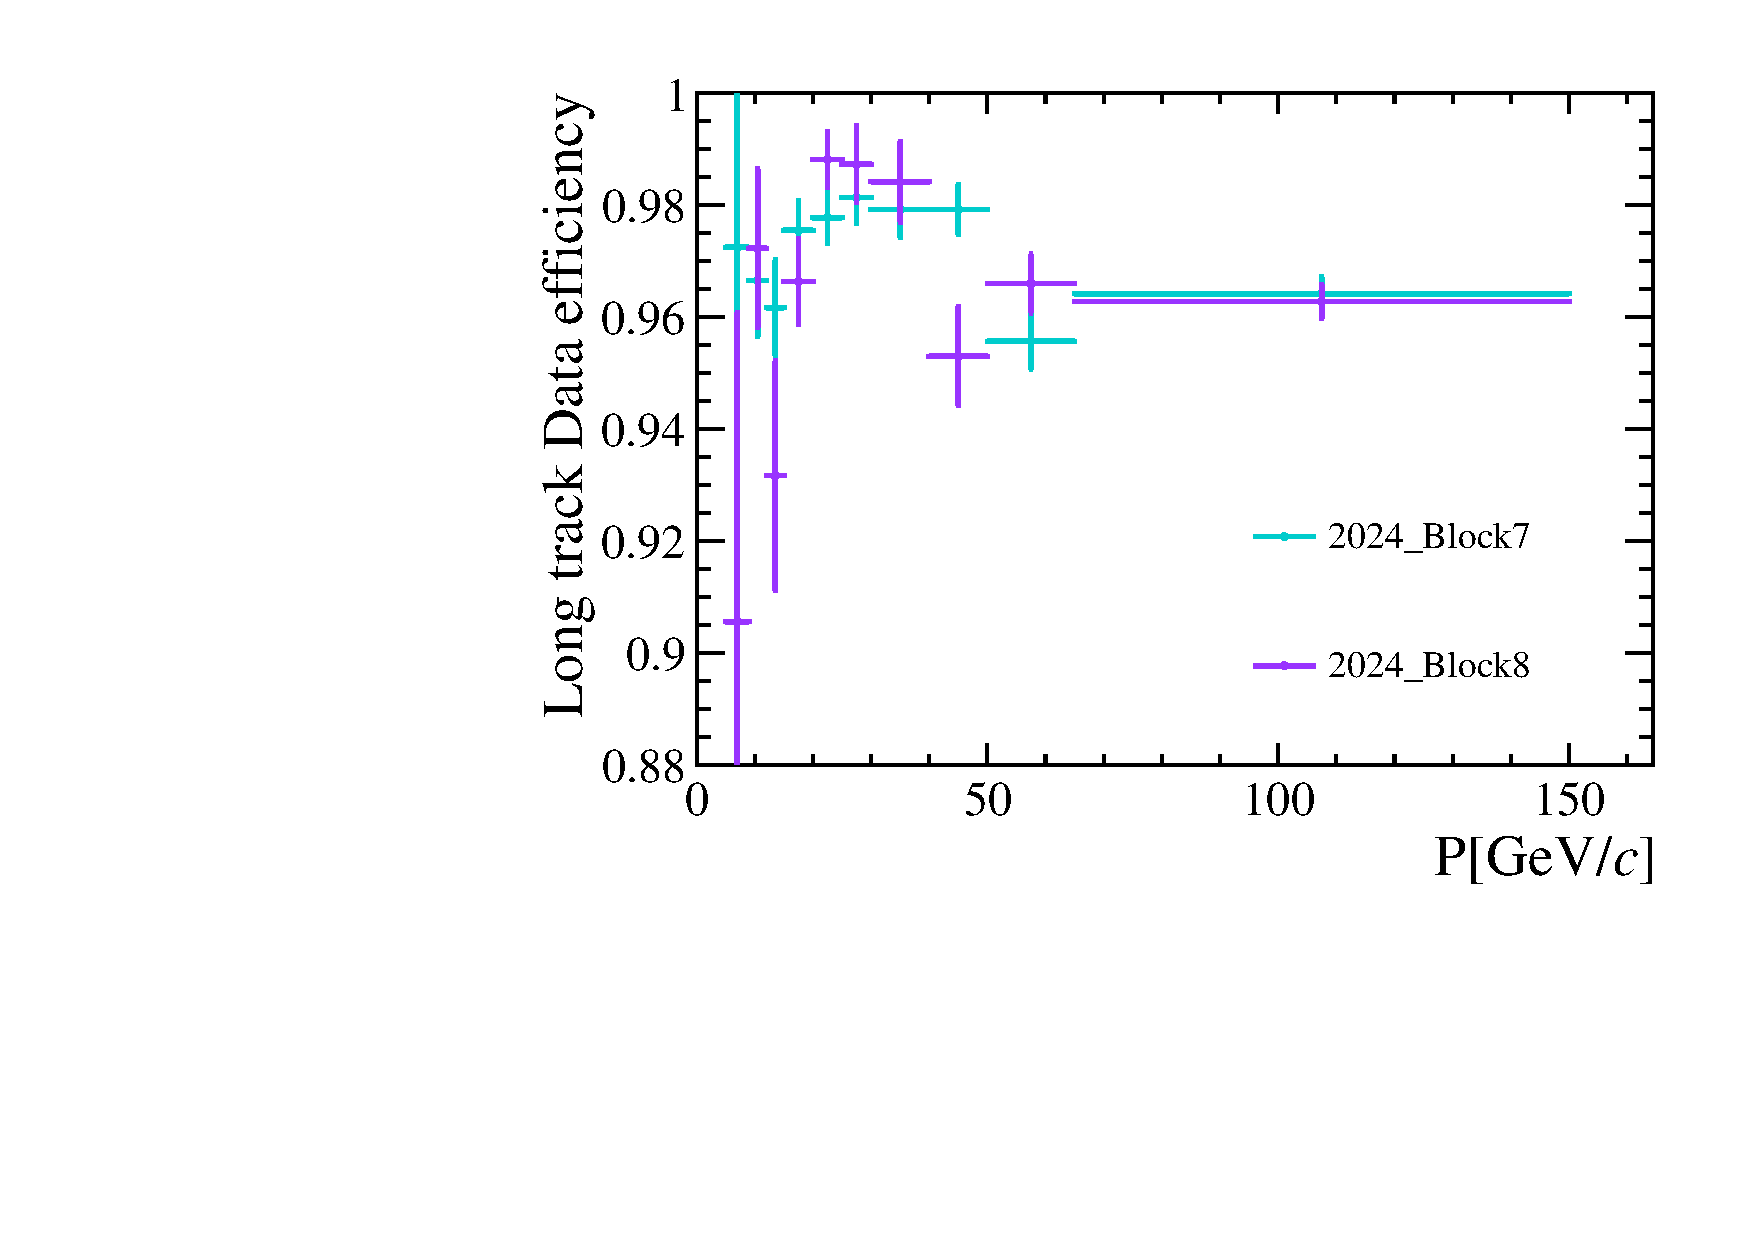
\includegraphics[width=0.75\textwidth]{Plots/trackeff_Data_MuonUT_P_not_respruced_samples.pdf}
    \end{subfigure}%
    \begin{subfigure}{0.5\textwidth}
      \centering
      
\includegraphics[width=0.75\textwidth]{Plots/trackeff_Data_MuonUT_P_respruced_samples.pdf}
    \end{subfigure}
    \begin{subfigure}{0.5\textwidth}
      \centering
      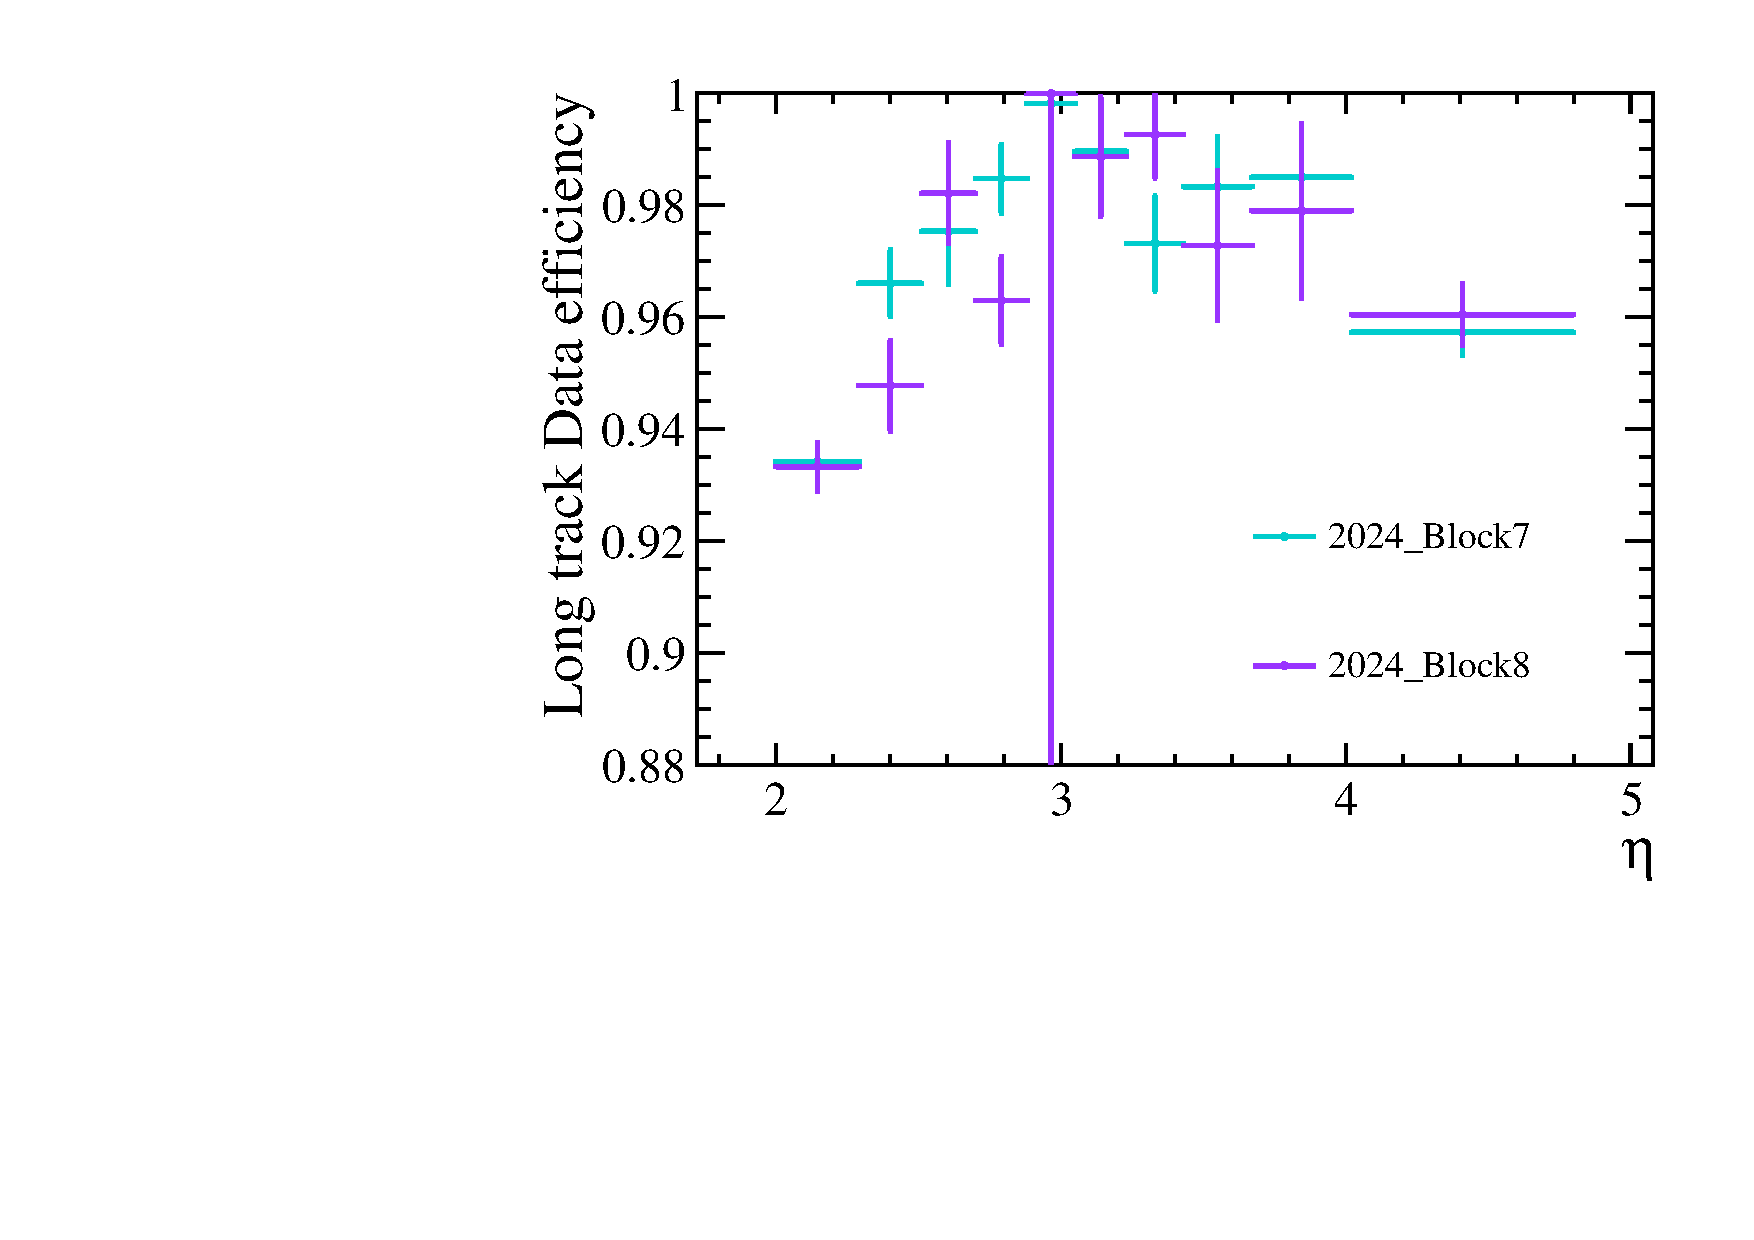
\includegraphics[width=0.75\textwidth]{Plots/trackeff_Data_MuonUT_ETA_not_respruced_samples.pdf}
    \end{subfigure}%
    \begin{subfigure}{0.5\textwidth}
      \centering
      
\includegraphics[width=0.75\textwidth]{Plots/trackeff_Data_MuonUT_ETA_respruced_samples.pdf}
    \end{subfigure}
  \end{figure}
  {MuonUT track efficiencies}
\end{frame}

\begin{frame}{Before and after resprucing data/MC ratio}
  \vspace{0.0cm}
  {\large Data/MC ratio}
  \begin{figure}[htb]
    \centering
    \begin{subfigure}{0.5\textwidth}
      \centering
      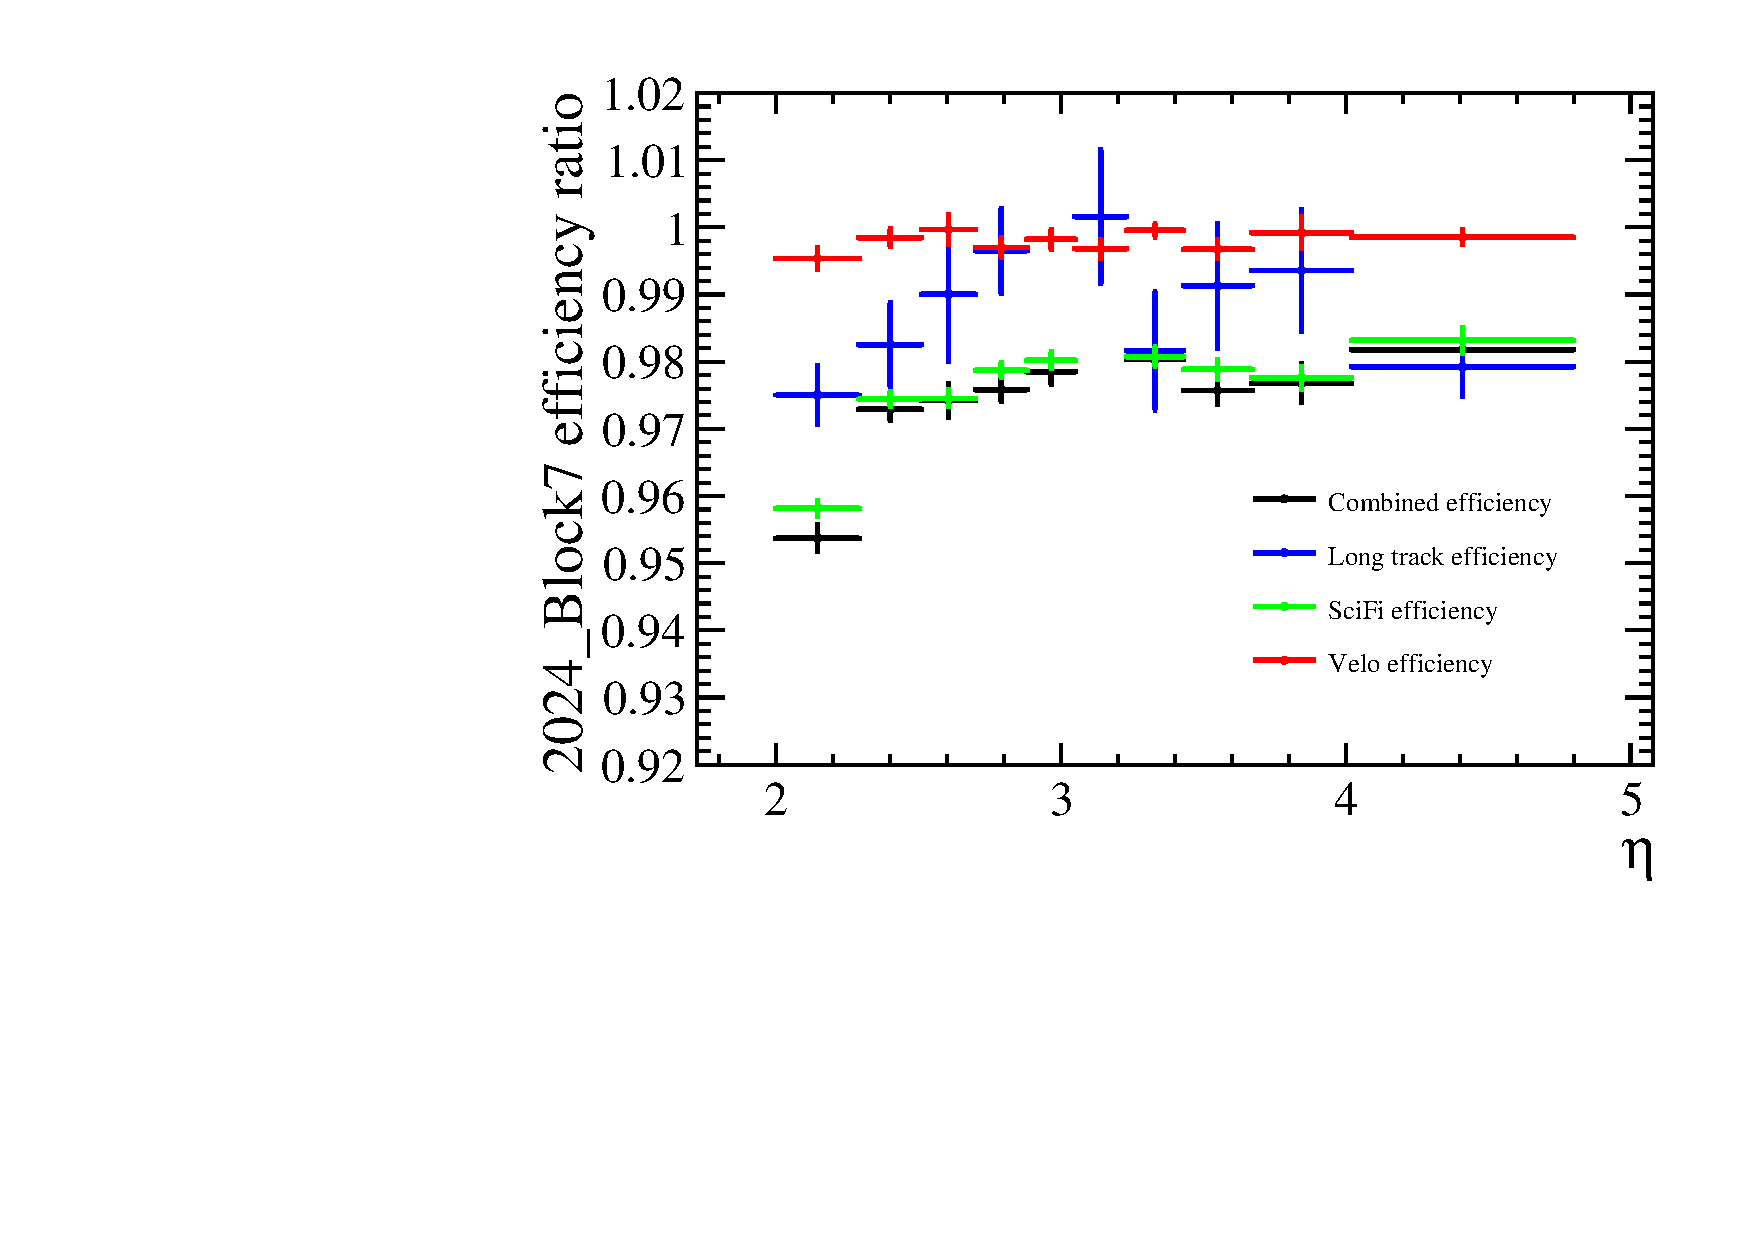
\includegraphics[width=1.0\textwidth]{Plots/trackeff_ratio_ETA_2024_Block7_not_respruced_samples.pdf}
    \end{subfigure}%
    \begin{subfigure}{0.5\textwidth}
      \centering
      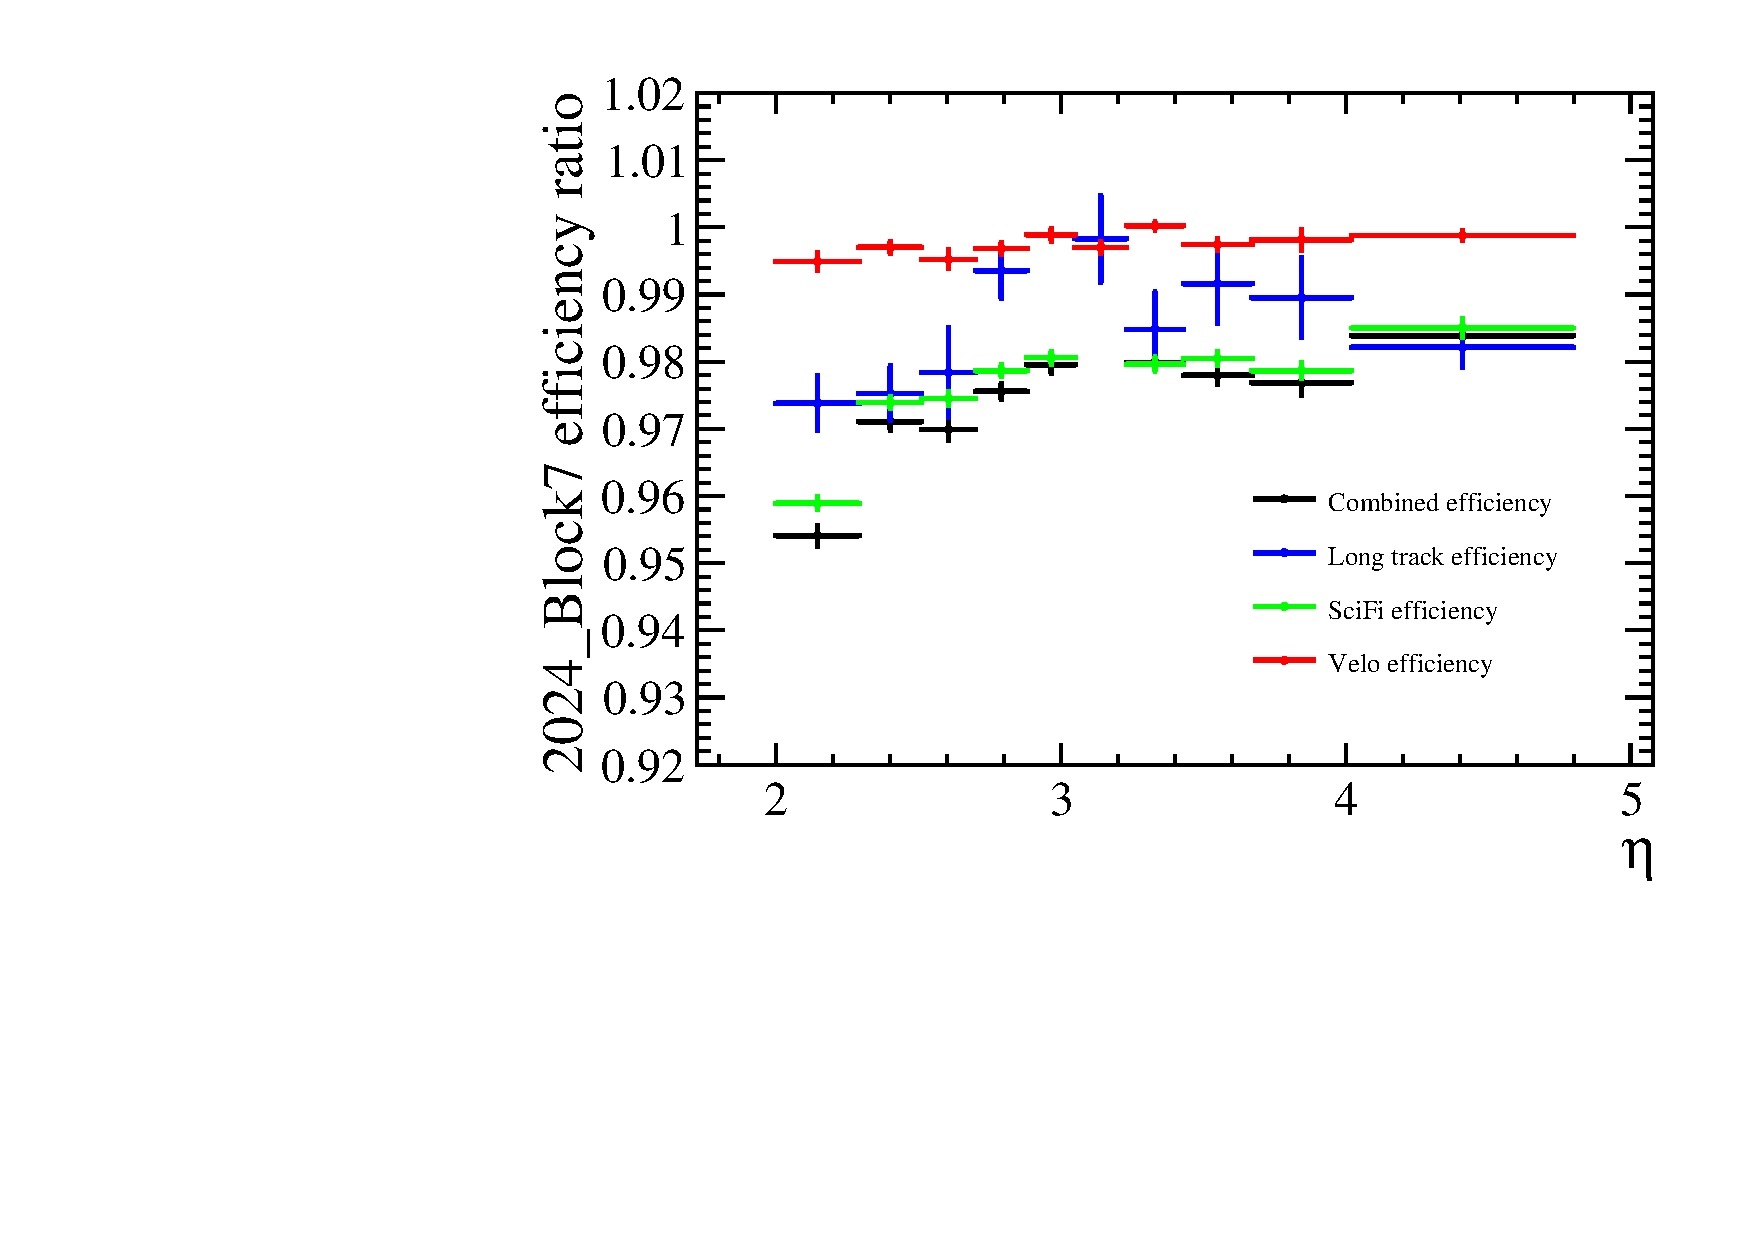
\includegraphics[width=1.0\textwidth]{Plots/trackeff_ratio_ETA_2024_Block7_respruced_samples.pdf}
    \end{subfigure}
  \end{figure}
  {Data/MC ratio for Combined/MuonUT track efficiencies block 7 in $\eta$}
\end{frame}

\begin{frame}{Before and after resprucing data/MC ratio}
  \vspace{0.0cm}
  {\large Data/MC ratio}
  \begin{figure}[htb]
    \centering
    \begin{subfigure}{0.5\textwidth}
      \centering
      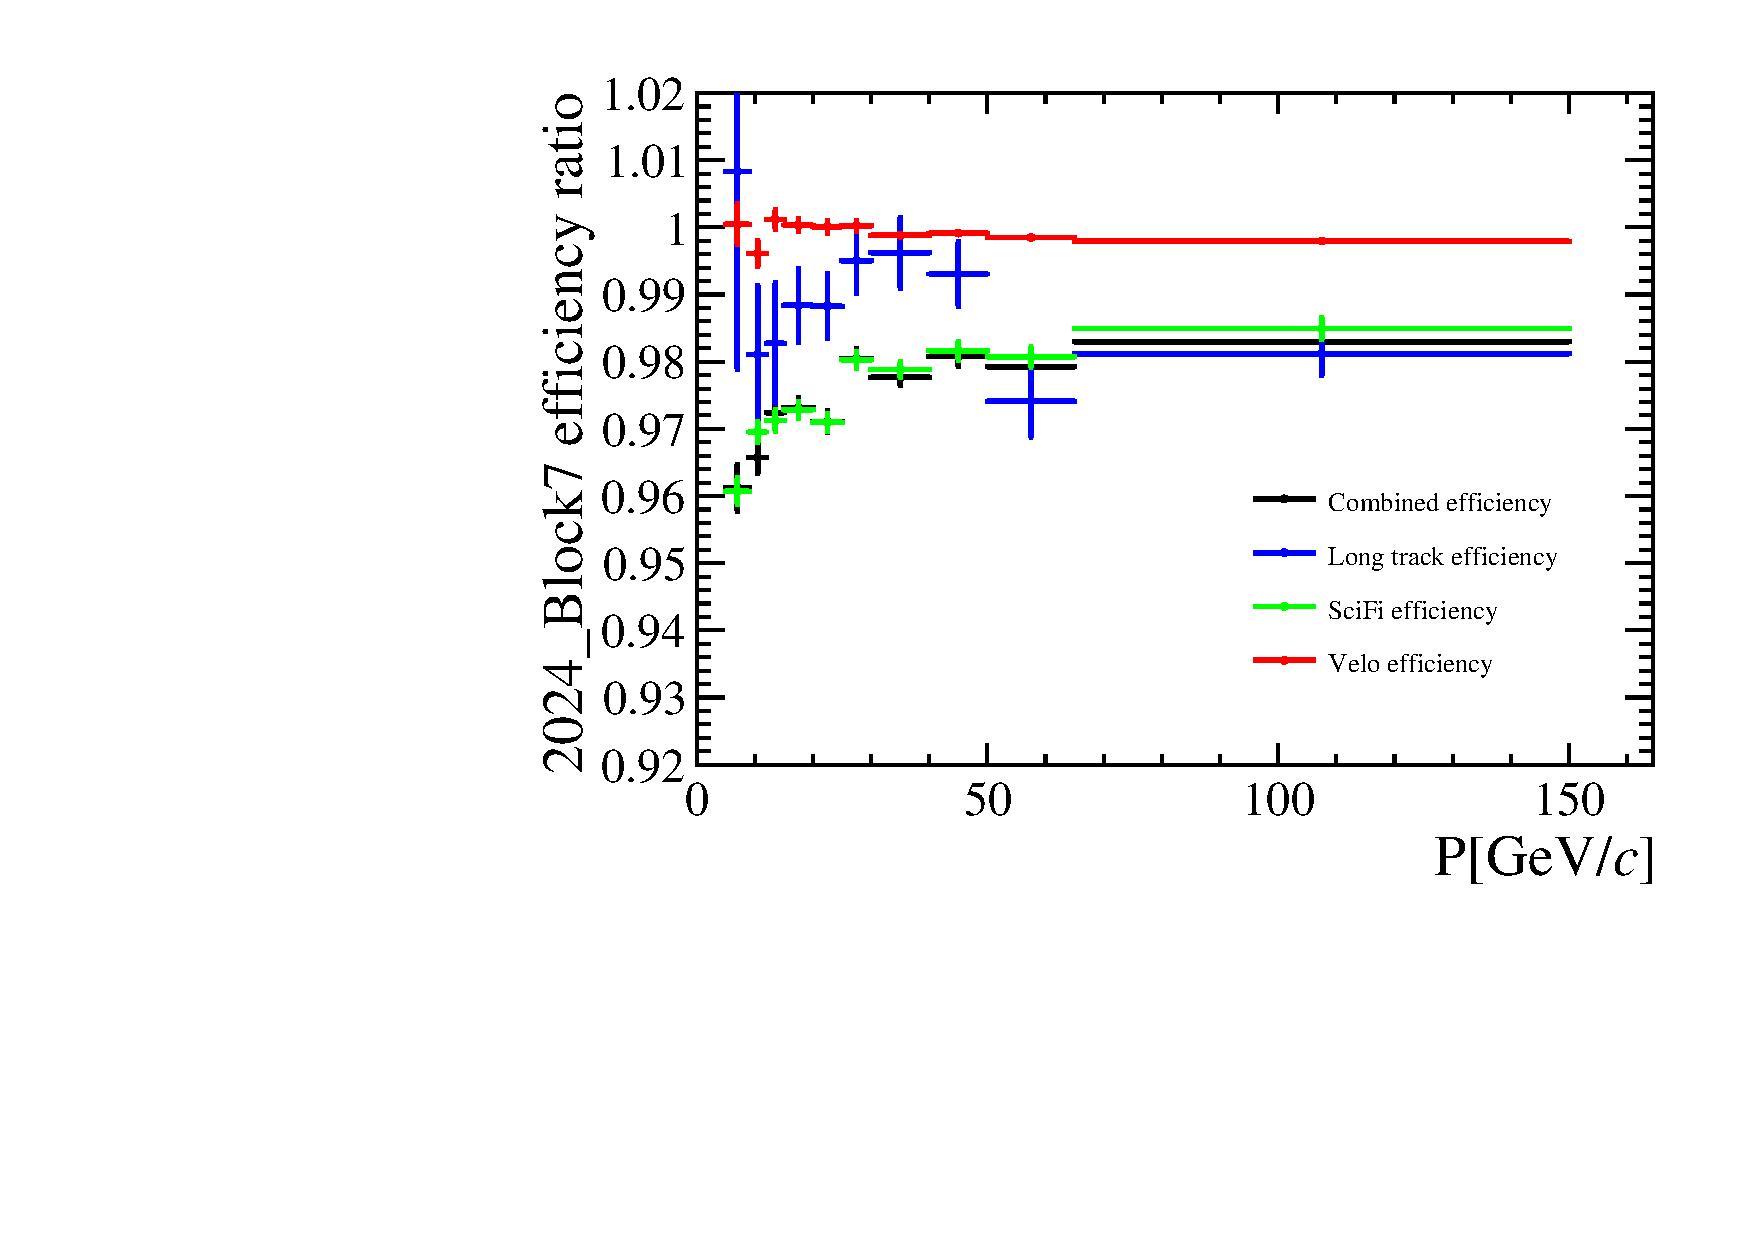
\includegraphics[width=1.0\textwidth]{Plots/trackeff_ratio_P_2024_Block7_not_respruced_samples.pdf}
    \end{subfigure}%
    \begin{subfigure}{0.5\textwidth}
      \centering
      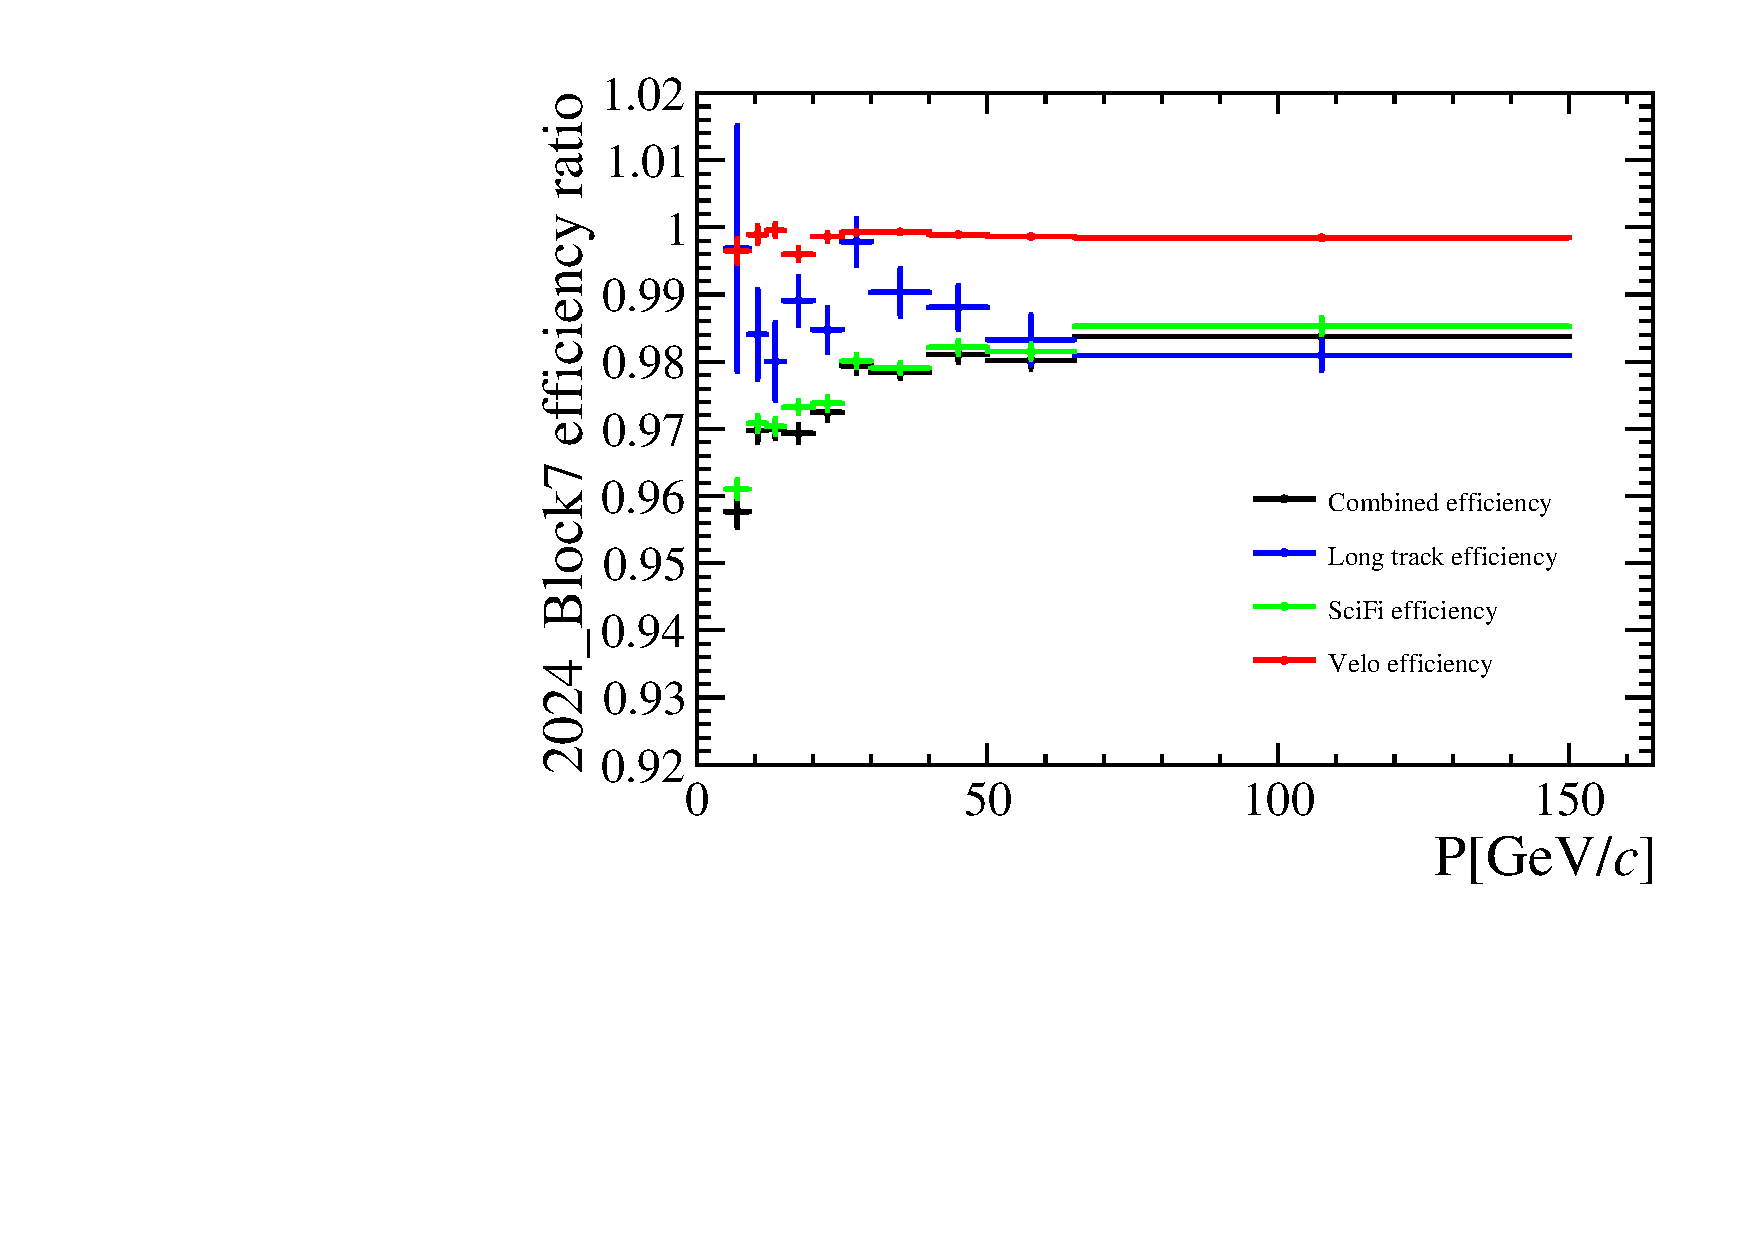
\includegraphics[width=1.0\textwidth]{Plots/trackeff_ratio_P_2024_Block7_respruced_samples.pdf}
    \end{subfigure}
  \end{figure}
  {Data/MC ratio for Combined/MuonUT track efficiencies block 7 in $p$}
\end{frame}

\begin{frame}{Before and after resprucing data/MC ratio}
  \vspace{0.0cm}
  {\large Data/MC ratio}
  \begin{figure}[htb]
    \centering
    \begin{subfigure}{0.5\textwidth}
      \centering
      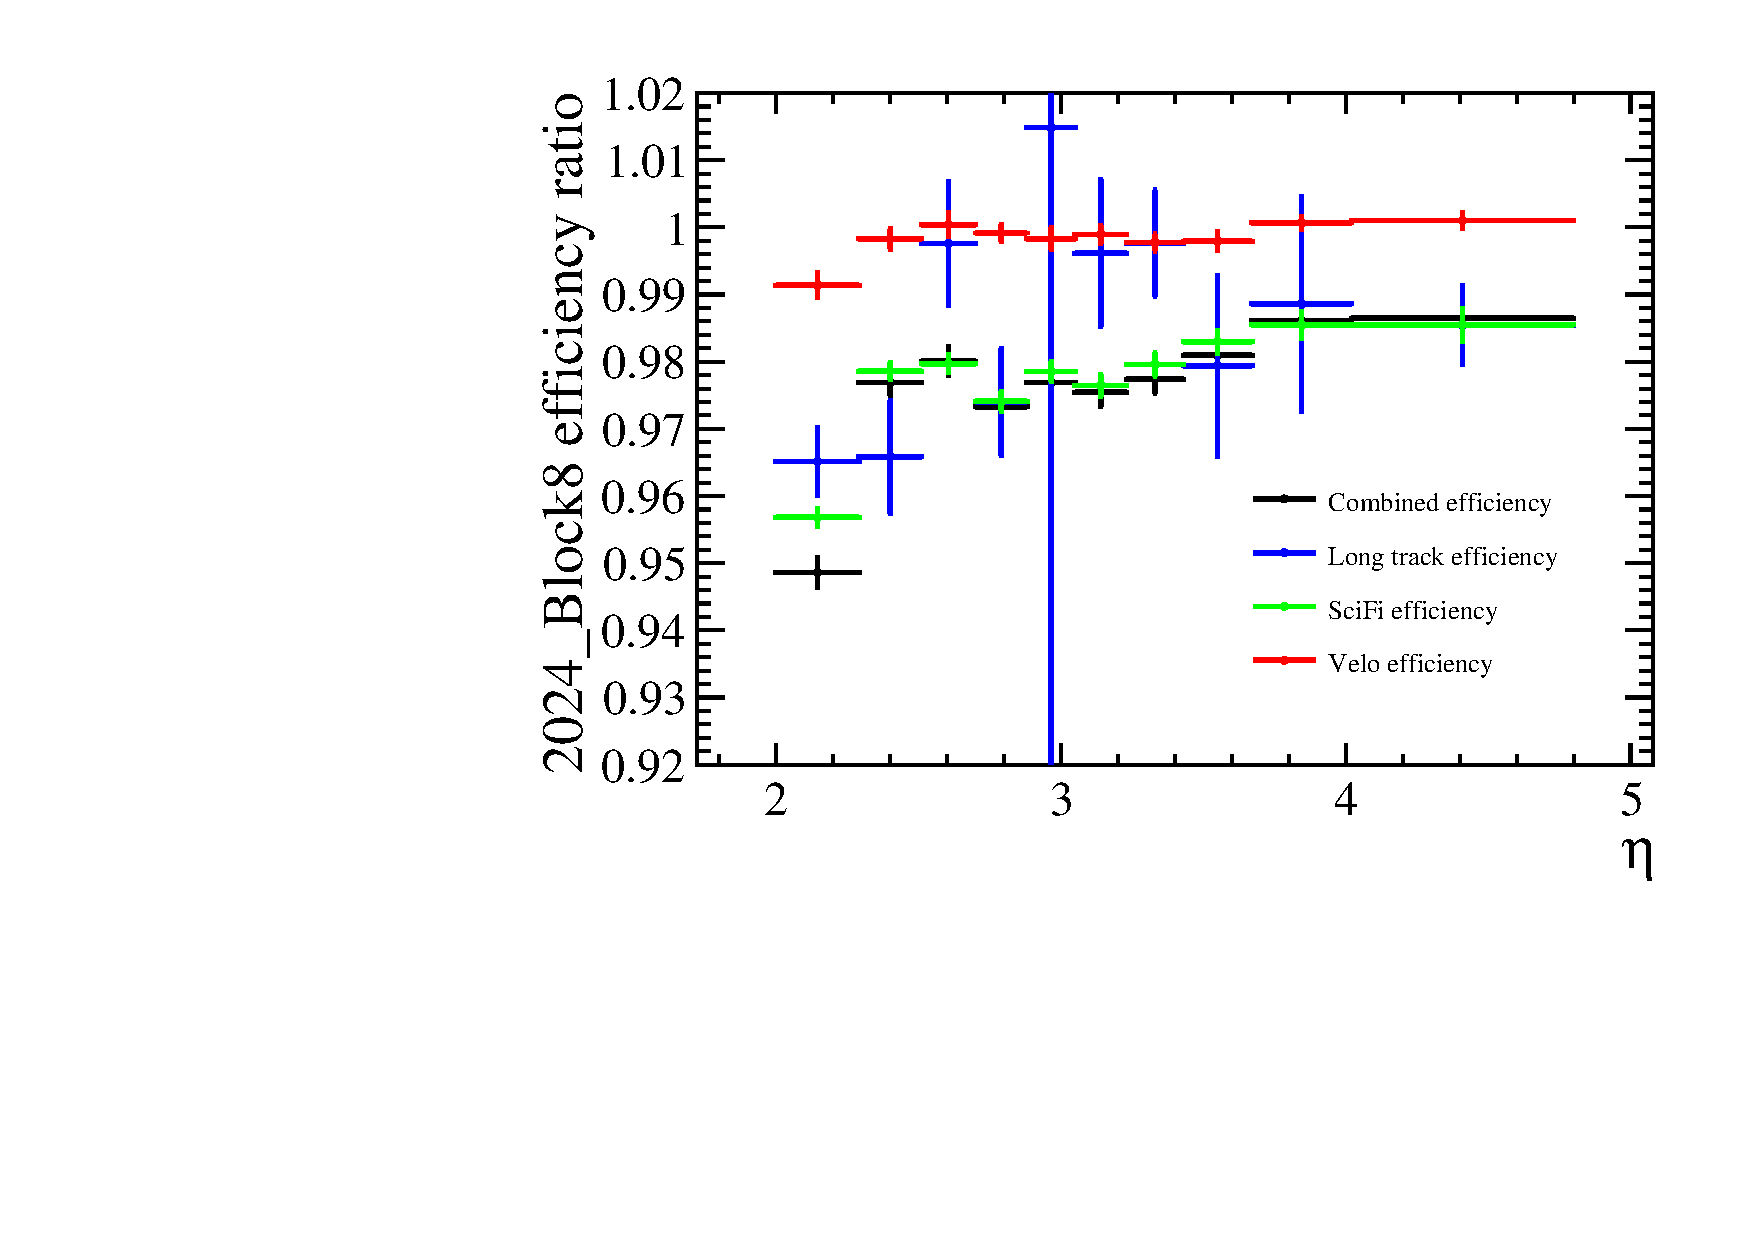
\includegraphics[width=1.0\textwidth]{Plots/trackeff_ratio_ETA_2024_Block8_not_respruced_samples.pdf}
    \end{subfigure}%
    \begin{subfigure}{0.5\textwidth}
      \centering
      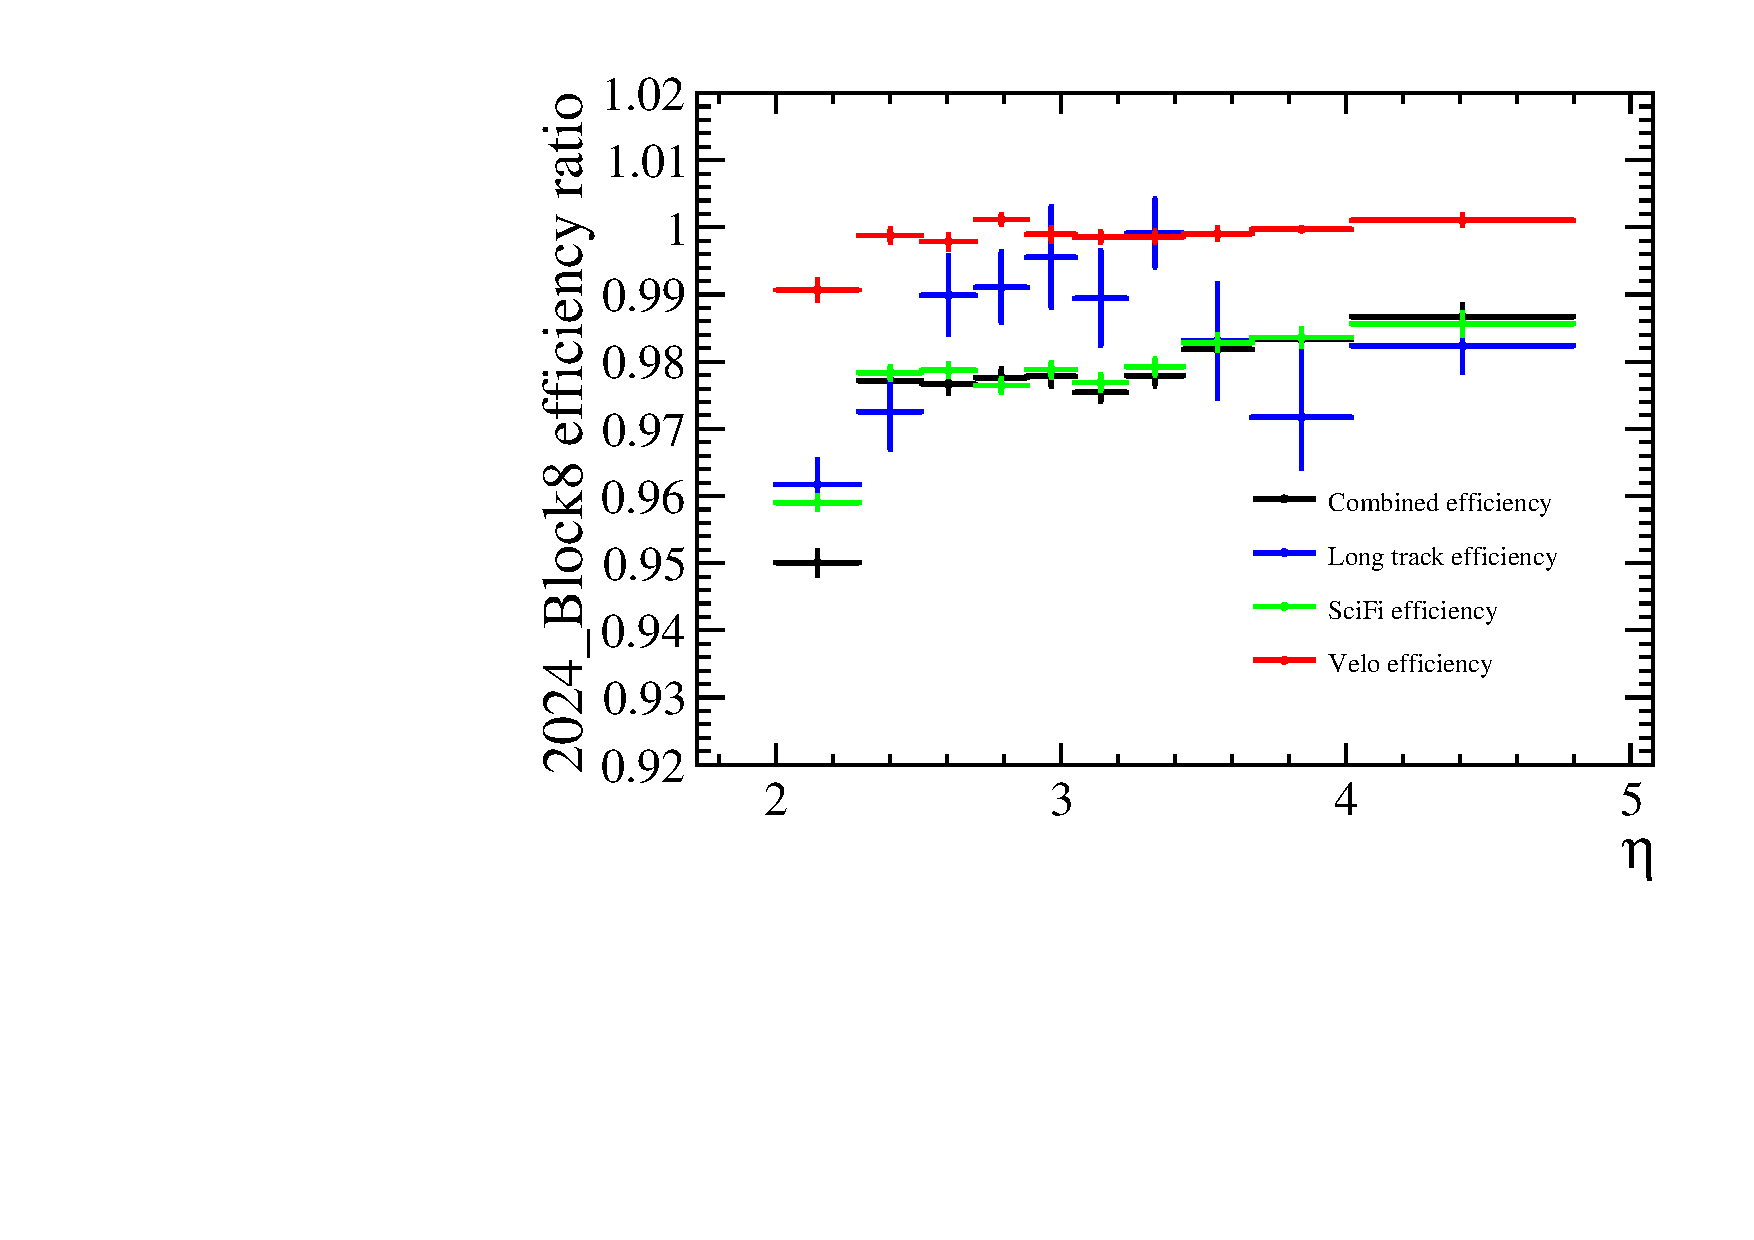
\includegraphics[width=1.0\textwidth]{Plots/trackeff_ratio_ETA_2024_Block8_respruced_samples.pdf}
    \end{subfigure}
  \end{figure}
  {Data/MC ratio for Combined/MuonUT track efficiencies block 8 in $\eta$}
\end{frame}

\begin{frame}{Before and after resprucing data/MC ratio}
  \vspace{0.0cm}
  {\large Data/MC ratio}
  \begin{figure}[htb]
    \centering
    \begin{subfigure}{0.5\textwidth}
      \centering
      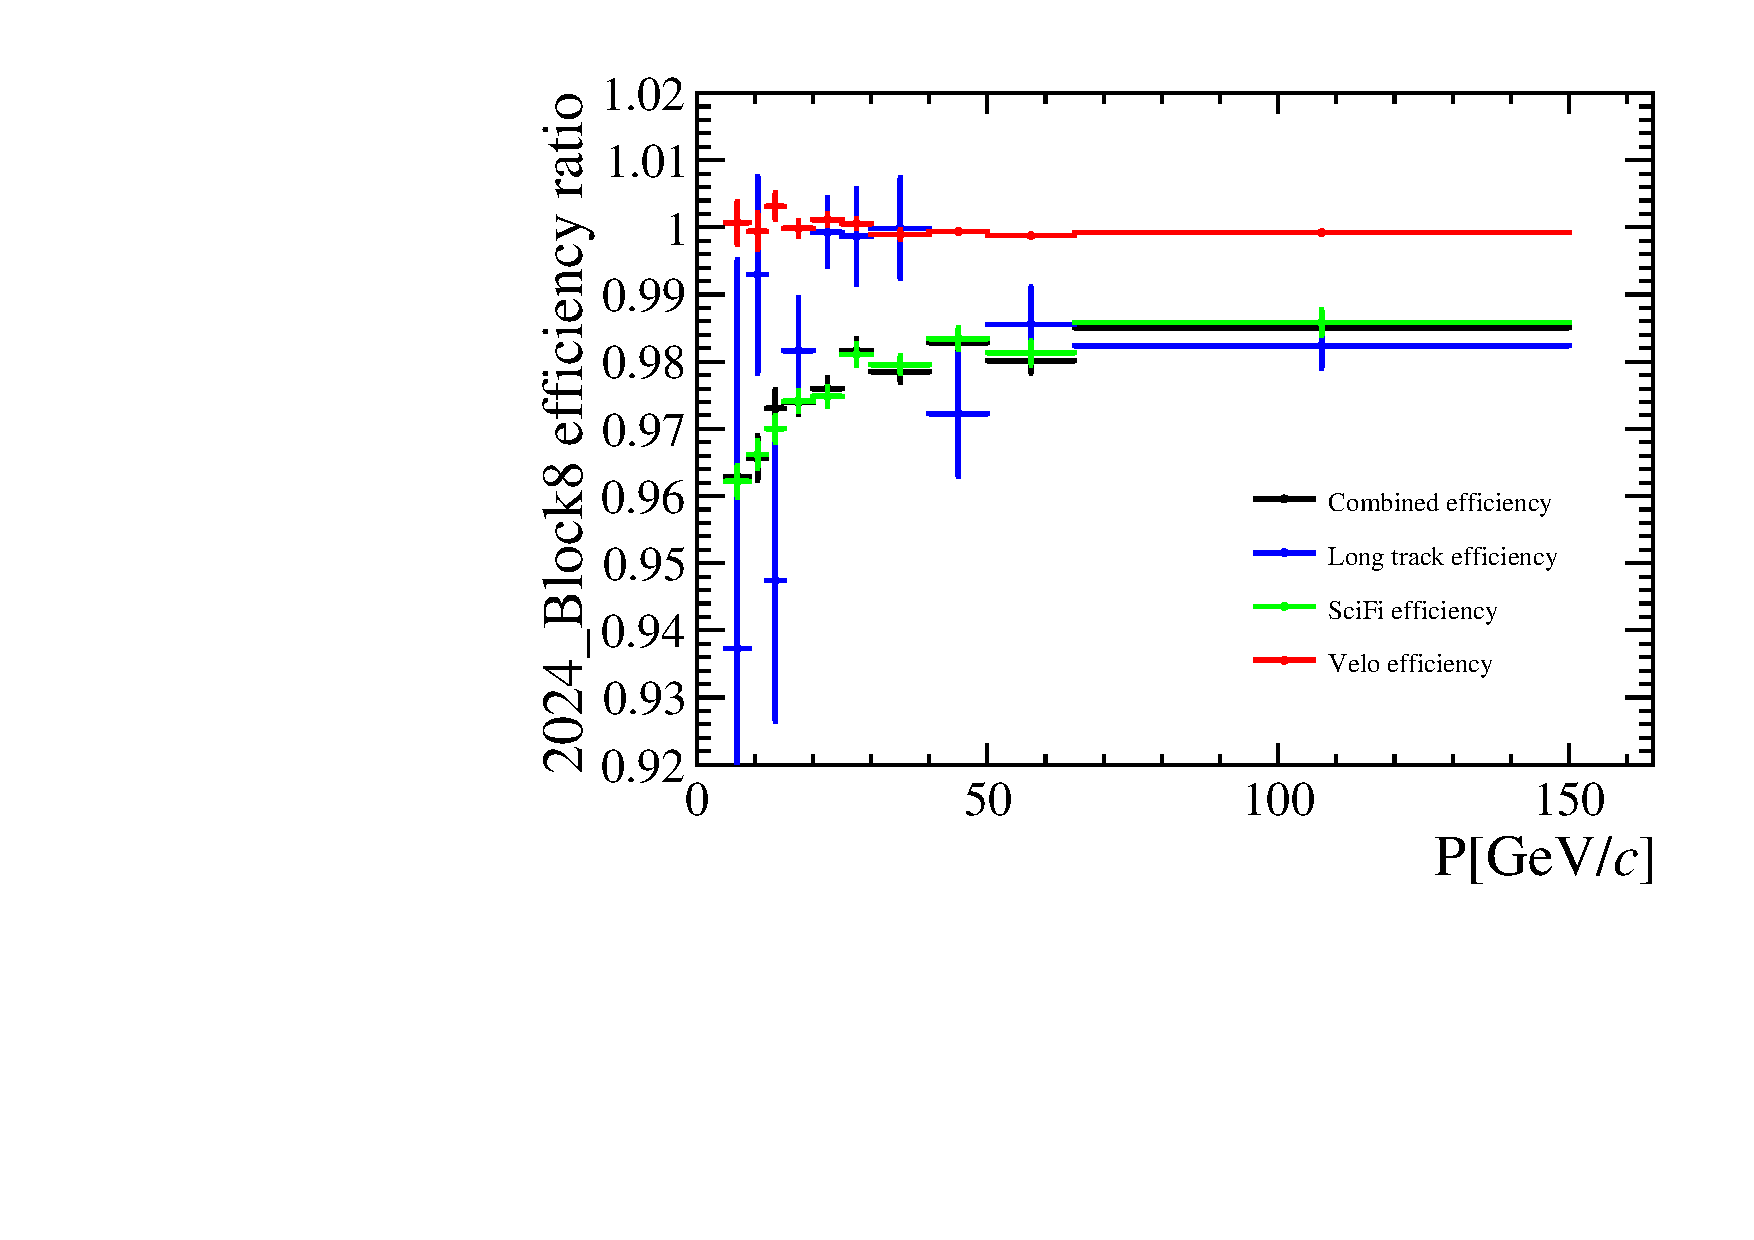
\includegraphics[width=1.0\textwidth]{Plots/trackeff_ratio_P_2024_Block8_not_respruced_samples.pdf}
    \end{subfigure}%
    \begin{subfigure}{0.5\textwidth}
      \centering
      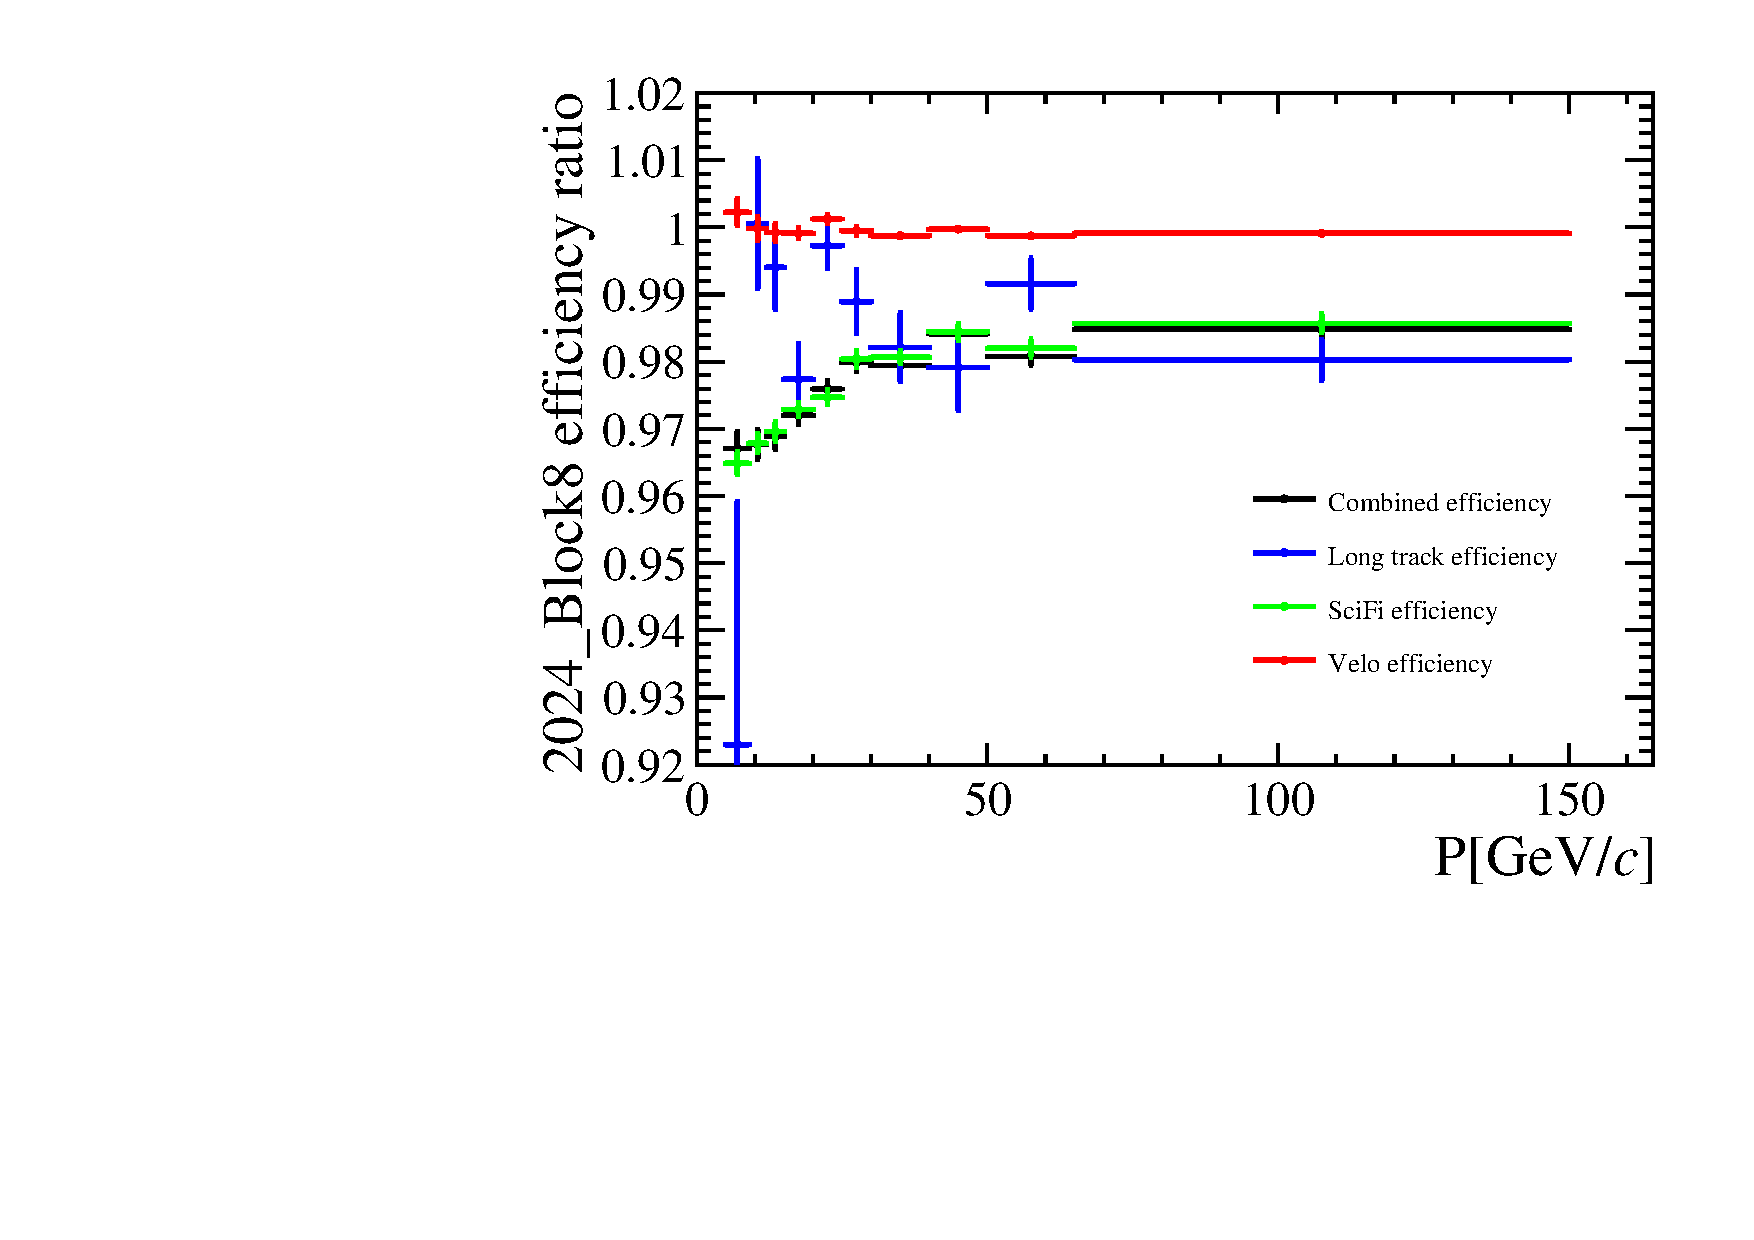
\includegraphics[width=1.0\textwidth]{Plots/trackeff_ratio_P_2024_Block8_respruced_samples.pdf}
    \end{subfigure}
  \end{figure}
  {Data/MC ratio for Combined/MuonUT track efficiencies block 8 in $p$}
\end{frame}

\begin{frame}{A/S week presentation outline}
  \vspace{0.0cm}
  {\large Is the following outline for A/S week fine?}
  \begin{enumerate}
    \setlength\itemsep{0.0em}
    \item{Introduction to track-and-probe method for tracking efficiencies}
    \begin{itemize}
      \item{VeloMuon, Downstream, MuonUT}
    \end{itemize}
    \item{List the datasets and MC samples}
    \item{Example of mass fit in TrackCalib2 to extract efficiency}
    \item{Show 1D projections in $p$ and $\eta$}
    \item{Explain what we provide to analysts:}
    \begin{itemize}
      \item{Data/MC ratio of tracking efficiencies}
      \item{2D binning in $p$ and $\eta$}
      \item{Statistical uncertainties from data/MC}
      \item{Systematic uncertainties, mainly from Combined-MuonUT discrepancy}
    \end{itemize}
    \item{Introduce 2D binning and GitLab release of corrections}
    \item{Discuss status of 2025 and block 1b?}
    \item{Present method for hadronic corrections}
    \item{Show hadronic correction results}
    \item{Anything else to discuss on hadronic corrections?}
  \end{enumerate}
\end{frame}

\end{document}
